\documentclass[12pt]{article}
\usepackage[margin=1in]{geometry}
\usepackage{amsmath,amssymb}
\usepackage{graphicx}
\usepackage{hyperref}
\usepackage{enumitem}
\usepackage{caption}
\usepackage{setspace}
\onehalfspacing
\graphicspath{{../../static/screenshots/}}

\title{专利三：量子干涉裁决与混币分流去匿名化方法与系统}
\author{申请人：ChainAML 项目}
\date{\today}

\begin{document}
\maketitle

\begin{abstract}
提出一种面向混币分流的量子干涉裁决方法与系统，基于金额守恒、等额聚类、时间协同与流守恒约束构造搜索空间，以 Grover 干涉放大满足约束的高风险组合，实现混币去匿名与证据链重建。
\end{abstract}

\section*{技术领域}
量子算法、图约束优化与反洗钱取证领域。

\section*{背景技术}
混币交易打散来源，导致传统追踪在多组合空间中的效率与解释性不足。

\section*{发明内容（概要）}
组合空间与约束建模 + 量子干涉裁决 + 匹配关系与置信度输出，支持“非法到合法”的路径重建与证据链生成。

\section*{附图说明}
图5：量子裁决流程图。\\
图6：结果可视化（分类饼图与交易明细表）。\\
图7：Step III 页面截图（量子干涉）占位。\\
图8：分类列表页面截图占位。

\section*{具体实施方式}
\subsection*{约束建模与组合空间}
解析混币交易集 $M$，输入集合 $I$、输出集合 $O$、金额向量 $a$；构造组合空间 $\Omega$（路径/地址组合）。

\subsection*{约束条件}
金额守恒：
\begin{equation}
\sum\limits_{i\in I} a_i = \sum\limits_{o\in O} a_o
\end{equation}
等额输出聚类：对 $O$ 的金额做聚类得到典型等额组 $O_k$；时间协同与共同输入关联；图流保守：
\begin{equation}
\sum f_{\text{in}}(v) = \sum f_{\text{out}}(v)
\end{equation}

\subsection*{量子干涉裁决}
初态：
\begin{equation}
|s\rangle=\frac{1}{\sqrt{N}}\sum\limits_{x\in \Omega}|x\rangle
\end{equation}
Oracle 标记满足约束且风险评分超阈的组合并相位翻转；扩散算子：
\begin{equation}
D=2|s\rangle\langle s|-I,\ \ G=D\cdot O
\end{equation}
迭代 $r$ 次放大目标集合：
\begin{equation}
\Pr(\text{hit})=\sin^2((2r+1)\theta),\ \ \sin^2\theta=\frac{|\mathcal{M}|}{N}
\end{equation}
风险评分：
\begin{equation}
\mathrm{score}(x)=\lambda_1 z_{\mathrm{time}}+\lambda_2 c_{\mathrm{path}}+\lambda_3 h_{\mathrm{mix}}+\lambda_4 p_q
\end{equation}

\subsection*{“非法到合法”的路径与追踪}
非法来源经混币打散为等额输出并跨地址/时间分散，试图断开来源关联；本方法以时间共振定位协同行为、黏菌主路径确定拓扑、量子裁决在组合空间中放大满足约束的目标组合，并以水印记录关键跳点，重建 \(I\rightarrow O\) 的候选映射与置信度。

\subsection*{实施环境与数据}
同专利一说明；权重 $\lambda_i$ 依据历史真值集调参，迭代步数 $r$ 按 \(\sin^2\theta\) 自适应选择。

\section*{权利要求书}
\begin{enumerate}[label=\arabic*.]
\item 一种量子干涉裁决方法用于混币分流去匿名化，包括：构造组合空间与约束集合；以 Grover 干涉放大满足约束且评分超阈的目标组合；输出匹配关系与置信度。
\item 根据权利要求1所述方法，其中风险评分函数与权重 $\lambda_i$ 通过标注数据优化。
\item 根据权利要求1所述方法，其中等额输出聚类采用密度或间隔阈值法形成 $O_k$。
\item 一种实现上述方法的系统，包括组合空间生成、约束计算、量子裁决与匹配输出模块，结构如图5。
\end{enumerate}

\section*{附图（放置截图文件）}
\begin{figure}[h]
  \centering
  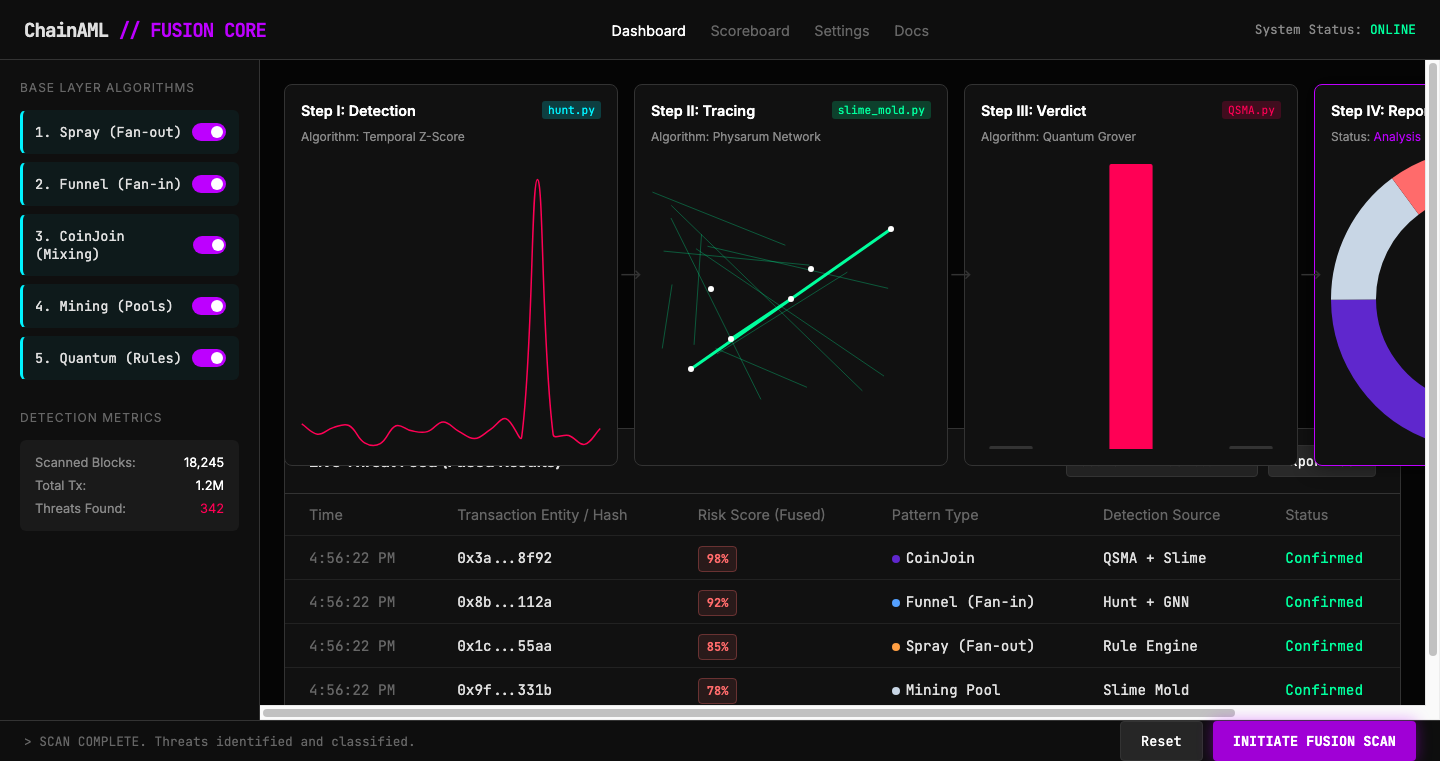
\includegraphics[width=0.9\linewidth]{step3.png}
  \caption{Step III：量子干涉裁决截图（占位）}
\end{figure}
\begin{figure}[h]
  \centering
  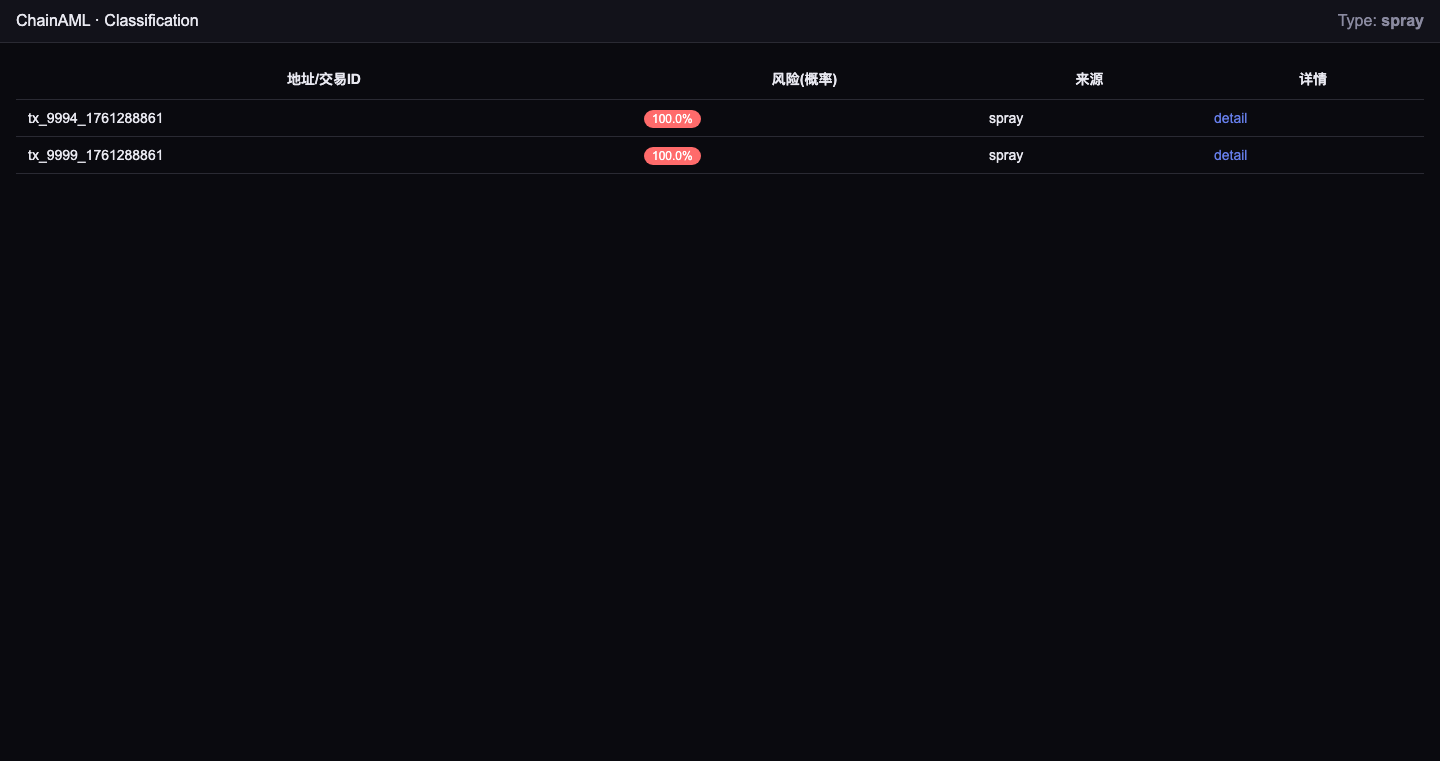
\includegraphics[width=0.9\linewidth]{classification_list.png}
  \caption{分类列表页面截图（占位）}
\end{figure}

\end{document}

